Let $\alpha$ be a real number satisfying $0 < \alpha < 180$.
For Leo's birthday, Frieder has placed $2025$ gnomes at arbitrary points inside his garden.
No three gnomes are collinear and no two gnomes coincide.
Each gnome has a field of view spanning $\alpha$ degrees (including the boundary).
After Frieder places the gnomes down, Leo wants to rotate the gnomes such that, for each gnome,
the number of other gnomes it sees is different.
Determine all values of $\alpha$ for which Leo can achieve this, regardless of how the gnomes are placed.

\begin{center}
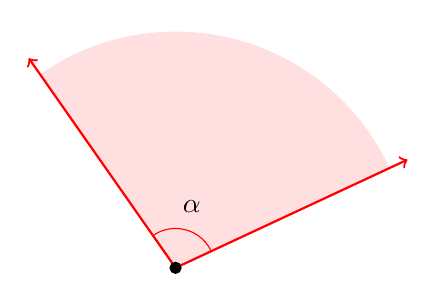
\begin{tikzpicture}
% Define the origin and angles
\coordinate (O) at (0,0);
\def\angleA{25}
\def\angleB{125}
\def\radius{3}
\def\angradius{0.5}

% Fill the sector between the rays
\filldraw[fill=pink, draw=none, opacity=0.5] 
    (O) -- (\angleA:\radius) arc (\angleA:\angleB:\radius) -- cycle;
    
    
\draw[red] 
    (O) -- (\angleA:\angradius) arc (\angleA:\angleB:\angradius) -- cycle;

% Draw the red rays
\draw[red, thick, ->] (O) -- (\angleA:\radius+0.25);
\draw[red, thick, ->] (O) -- (\angleB:\radius+0.25);

% Draw the black point
\filldraw[black] (O) circle (2pt);

% Label the angle alpha
\node at (75:0.8) {$\alpha$};
\end{tikzpicture}\\
\caption{\emph{An example of the field of view of a gnome. It extends infinitely between the boundary rays.}}
\end{center}
